%%%%%%%%%%%%%%%%%%%%%%%%%%%%%%%%%%%%%%%%%
% University Assignment Title Page 
% LaTeX Template
% Version 1.0 (27/12/12)
%
% This template has been downloaded from:
% http://www.LaTeXTemplates.com
%
% Original author:
% WikiBooks (http://en.wikibooks.org/wiki/LaTeX/Title_Creation)
%
% License:
% CC BY-NC-SA 3.0 (http://creativecommons.org/licenses/by-nc-sa/3.0/)
% 
% Instructions for using this template:
% This title page is capable of being compiled as is. This is not useful for 
% including it in another document. To do this, you have two options: 
%
% 1) Copy/paste everything between \begin{document} and \end{document} 
% starting at \begin{titlepage} and paste this into another LaTeX file where you 
% want your title page.
% OR
% 2) Remove everything outside the \begin{titlepage} and \end{titlepage} and 
% move this file to the same directory as the LaTeX file you wish to add it to. 
% Then add \input{./title_page_1.tex} to your LaTeX file where you want your
% title page.
%
%%%%%%%%%%%%%%%%%%%%%%%%%%%%%%%%%%%%%%%%%

%----------------------------------------------------------------------------------------
%	PACKAGES AND OTHER DOCUMENT CONFIGURATIONS
%----------------------------------------------------------------------------------------

\documentclass[12pt]{article}
\usepackage{graphicx}
\begin{document}

\begin{titlepage}

\newcommand{\HRule}{\rule{\linewidth}{0.5mm}} % Defines a new command for the horizontal lines, change thickness here


 
%----------------------------------------------------------------------------------------

\center % Center everything on the page
 
%----------------------------------------------------------------------------------------
%	HEADING SECTIONS
%----------------------------------------------------------------------------------------


%----------------------------------------------------------------------------------------
%	LOGO SECTION
%----------------------------------------------------------------------------------------


\includegraphics{logo_epfl-eps-converted-to}\\[1cm] % Include a department/university logo - this will require the graphicx package

%\textsc{\LARGE \'Ecole Polytechnique F\'ed\'erale de Lausanne}\\[1.5cm] % Name of your university/college
\textsc{\Large Biological Modeling of Neural Networks}\\[0.5cm] % Major heading such as course name

%----------------------------------------------------------------------------------------
%	TITLE SECTION
%----------------------------------------------------------------------------------------

\HRule \\[0.4cm]
{ \huge \bfseries Hopfield Model}\\[0.4cm] % Title of your document

\textsc{\large Storage of Sequences of patterns in asymetric hopfield networks with delayed synapses}\\[0.5cm] % Minor heading such as course title

\HRule \\[1.5cm]

%----------------------------------------------------------------------------------------
%	AUTHOR SECTION
%----------------------------------------------------------------------------------------

\begin{flushright}
\large Miryam \textsc{Chaabouni}

\large Joseph \textsc{Lemaitre}\\ % Your name

\end{flushright}


% If you don't want a supervisor, uncomment the two lines below and remove the section above
%\Large \emph{Author:}\\
%John \textsc{Smith}\\[3cm] % Your name

%----------------------------------------------------------------------------------------
%	DATE SECTION
%----------------------------------------------------------------------------------------

%{\large \today}\\[3cm] % Date, change the \today to a set date if you want to be precise

\vfill % Fill the rest of the page with whitespace

\end{titlepage}

\section{Exercise 1}
\subsection{Exercise 1.1}
\begin{center}
    \begin{figure}
    \caption{$g(r)$ for 10K steps}\label{1}
    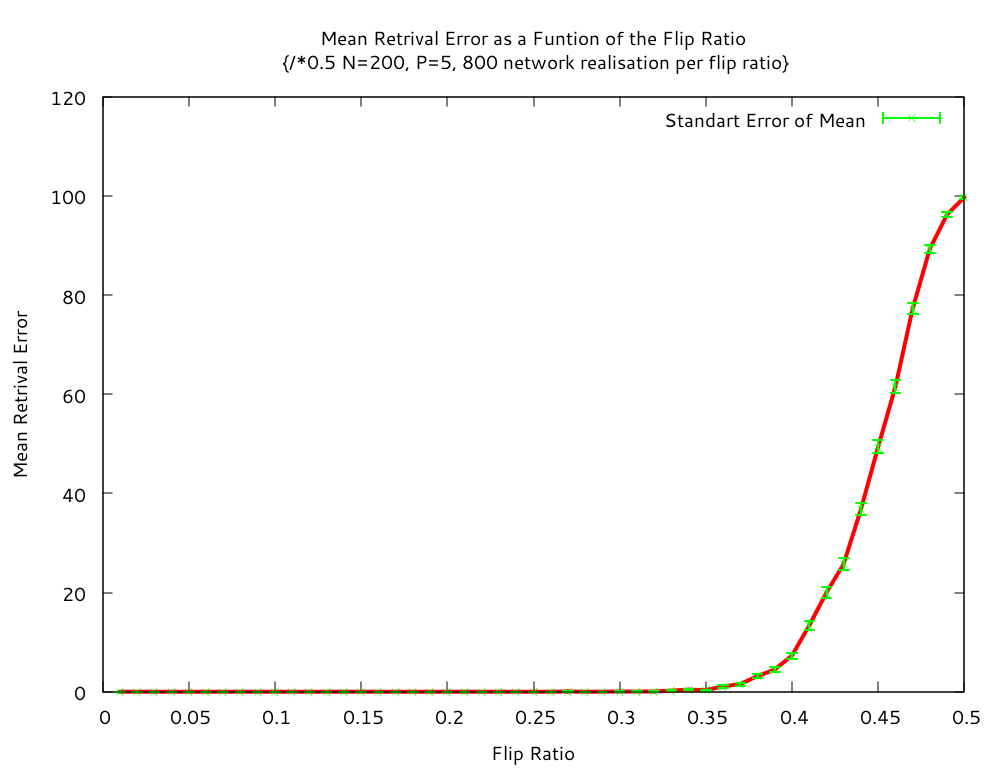
\includegraphics[scale=0.7]{img/ex11.png}
    \end{figure}
\end{center}

\subsection{Exercise 1.2}
\begin{center}
\begin{math}
    \begin{array}{|l|c|c|c|}
    \hline
    N & 100 & 250 & 500 \\ \hline
    P_{max} & 17 & 39 &  \\ \hline
    \alpha_{max} & 0.17 & 0.156 & - \\ \hline
    \alpha_{th} & - & - & - \\ \hline
    \end{array}
\end{math}
\end{center}

\section{Exercise 2}
\subsection{Exercise 2.2}
We used the heaviside filter function.
0.7 : 0->1->3, blocked at 3
0.8 : 0->1->3->4, blocked at 4
0.9 : sequencial behaviour

Definition of sequencial behaviour : all visited, equivalent to not more than 10 in the same
state. We found $\lambda_{min} = 0.9$ (lot of try. Some time work some time not).

For lamda max : sequencial behaviour : all state a visited with a overlap of 1, one after each other.
We found $\lambda_{min} = 3.6$
\subsection{Exercice 2.3}


\end{document}